\usepackage{placeins}
\usepackage{float}
\documentstyle[12pt,graphicx]{article}
\pagestyle{plain}
\baselineskip 18pt
\textwidth 6.5in
\textheight 7.8in
\oddsidemargin 0.1in
\evensidemargin 0.1in
\topmargin 0.3in
\parindent 0pt
\renewcommand{\thesubsection}{\thesection.\alph{subsection}}
\newcommand{\beq}{\begin{equation}}
\newcommand{\eeq}{\end{equation}}

\begin{document}

\title{Homework 3 - Spectral Method}
\author{Quynh Nguyen}
\maketitle


Note: The zip folder include main c++ code in /comp/hw3/ and ROOT plot code in /root/macros. Code is compiled in g++ (clang) in Mac OSX. 



\section{Problem 1: T and H}



\subsection{Average and RMS}
\paragraph{}
\begin{center}
\begin{tabular}{l*{6}{c}r}

\hline
   & first year & second year & both  \\

\hline
T mean & 23.3115 & 23.4154 & 23.3635  \\
\sigma_T & 3.47185 & 3.33382 & 3.40393  \\
\hline
\hline
H mean & 41.5769 & 40.6145 & 41.0962  \\
\sigma_H & 2.78972 & 2.97524 & 2.92377  \\
\hline
\hline
\end{tabular} 
\end{center}

\subsection{FFT and power spectrum}
\paragraph{}
  Before FFT, the given T and H data was subtracted by their means to remove the DC mode in the Fourier transform. 
  Complex one-dimension FFTW3 routine was called to produce an 104 $\times$ 2 array of Fourier coefficients. The power spectrum is calculated by adding absolute value of  $\hat{f(k)} $ and  $\hat{f(-k)} $ for each k (efficiently the 1D k shell with bin size 2$\Pi$/104. The spectra are shown in Fig. \ref{polar}.

\paragraph{}
Explain: The temperature original data (blue plot in Fig. \ref{polar}) displays a dominant mode with period of one year. That mode gives the highest point the the Fourier transform. The secondary dominant mode is 2 times higher in frequency. This is the main fluctuation on top of the dominant seasonal mode. Other frequencies contribute a lot less power.
\paragraph{}
The humidity original data (red plot in Fig. \ref{polar}) is more spread out and contain no clear dominant frequency thus the spectrum is more even out.


\begin{figure}[!htbp]
\begin{center}
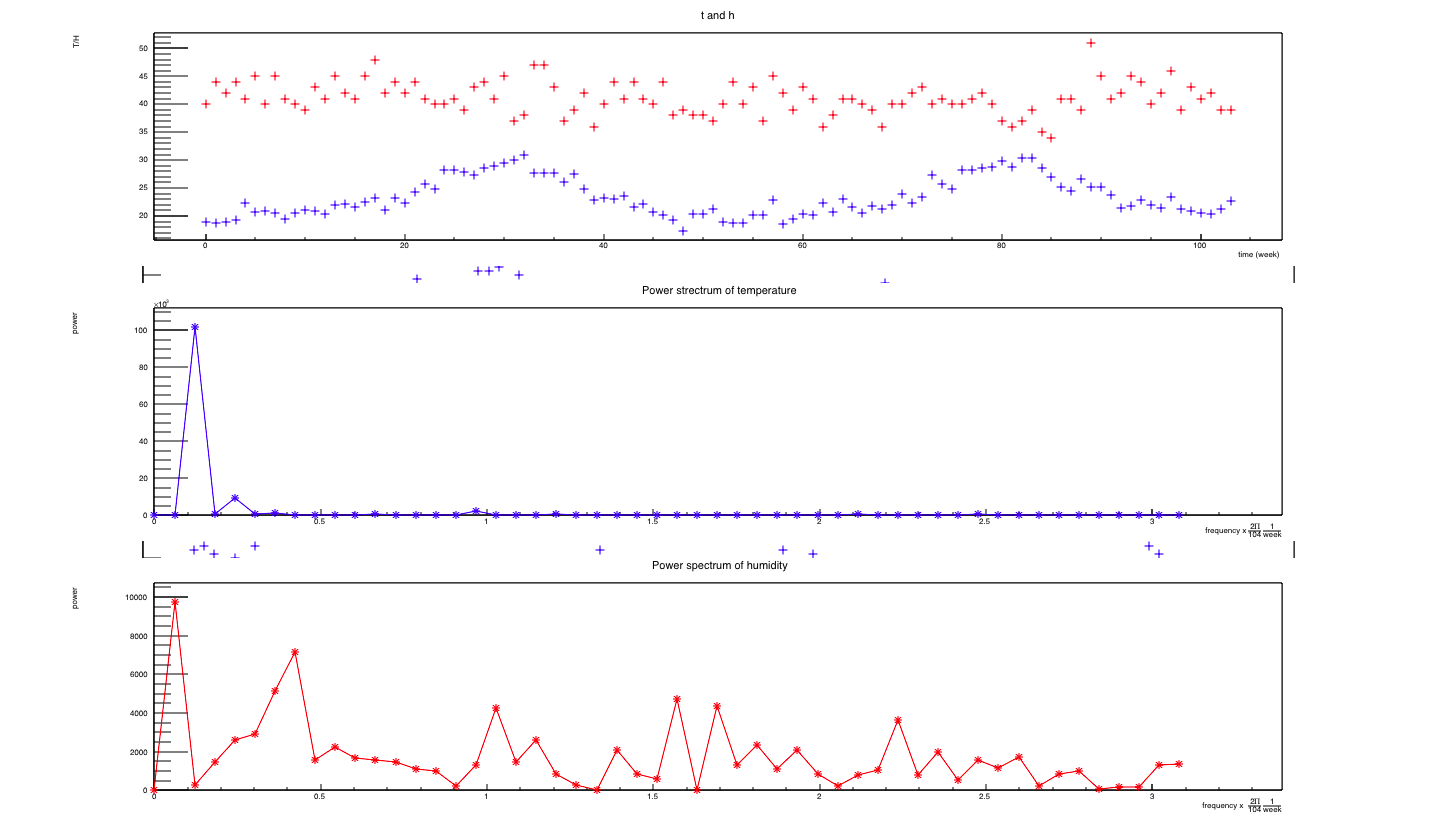
\includegraphics[height=17cm, width=17cm]{1_b.png}
\caption{Temperature and humid fluctuation and their power spectra}
\label{polar}
\end{center}
\end{figure}


\FloatBarrier
\subsection{Removing seasonal variation}
\paragraph{}
Seasonal variation has period of 1 year. Thus the corresponding frequency is  \pm2$\Pi$/104 x 2 =  $\Pi$/26. These frequencies were removed from the FFT which subsequently got inverse FFT to get fluctuation in T and H without seasonal variations. See Fig. \ref{sea}

\paragraph{}
Comparing fluctuation between H and T: RMS value of re-transformed T and H were optained.
\beq
T_{rms}/<T> \approx 0.90914/ 23.3635 \approx 0.039
\eeq
\beq
H_{rms}/<H> \approx 1.85591/ 41.0962 \approx 0.045
\eeq 
Thus, without seasonal variation, the humid data fluctuates more. This can be sean from Fig. \ref{sea}



\begin{figure}[!htbp]
 
\begin{center}
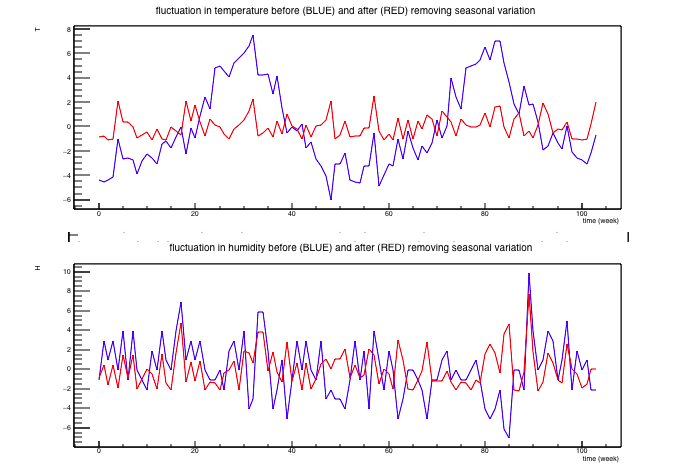
\includegraphics[height=17cm, width=17cm]{1_c_final.png}
\caption{Temperature and humid fluctuation with and without seasonal variation}
\label{sea}
\end{center}
\end{figure}


\FloatBarrier



\section{Problem 2: Gaussian Fields}



\subsection{implementation of FFT}
\paragraph{}
Main code in comp/hw3/problem2{\_}inmodule.cc. Plot code  /root/macros/hw3{\_}2.cc and hw3\_2c.cc
The data is ready in row major format and was fft by fftw3.

\subsection{Power spectrum}
\paragraph{}
In this problem, it is not neccesary to substract the mean before FFT because Gaussian fields have mean zero.




\paragraph{}
Log-Log plots of all three Gaussian fields power spectra are shown in blue in Fig. (\ref{2BC1}), (\ref{2BC2}) and (\ref{2BC3}). The 3D plots are linear. 

\begin{figure}[!htbp]
\centering
\begin{minipage}{.5\textwidth}
  \centering
  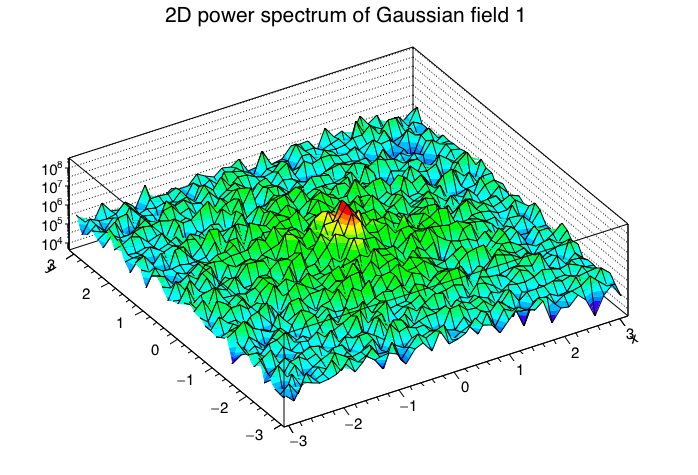
\includegraphics[width=1\linewidth]{gaus1color}
  \caption{Gaussian1}
  \label{1col}
  
\end{minipage}%
\begin{minipage}{.5\textwidth}
  \centering
  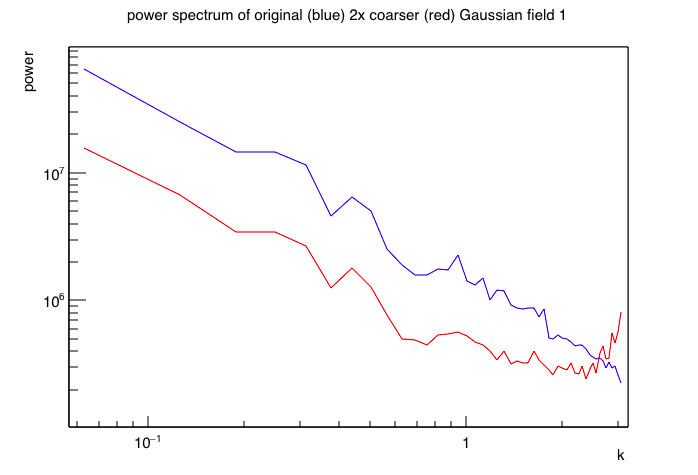
\includegraphics[width=1.1\linewidth]{2BC1}
  \caption{Gaussian1 before and after resampling. The plot remains linear feature up unil new Nyquist frequency $\Pi$/2}
  \label{2BC1}
\end{minipage}
\end{figure}

 
 \begin{figure}[!htbp]
\centering
\begin{minipage}{.5\textwidth}
  \centering
  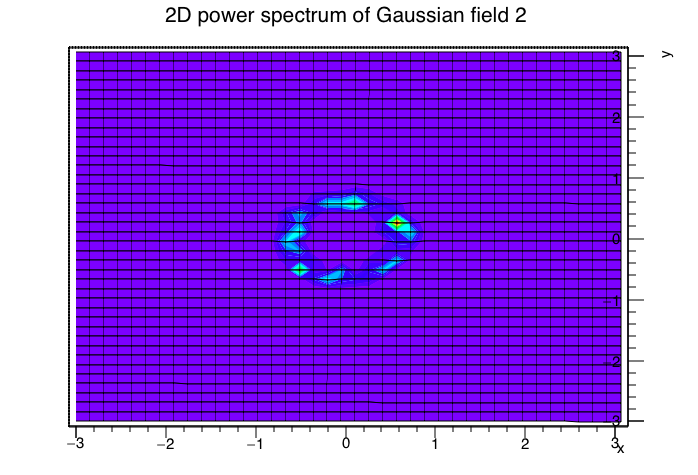
\includegraphics[width=1\linewidth]{gau2color}
  \caption{Gaussian2}
  \label{2col}
\end{minipage}%
\begin{minipage}{.5\textwidth}
  \centering
  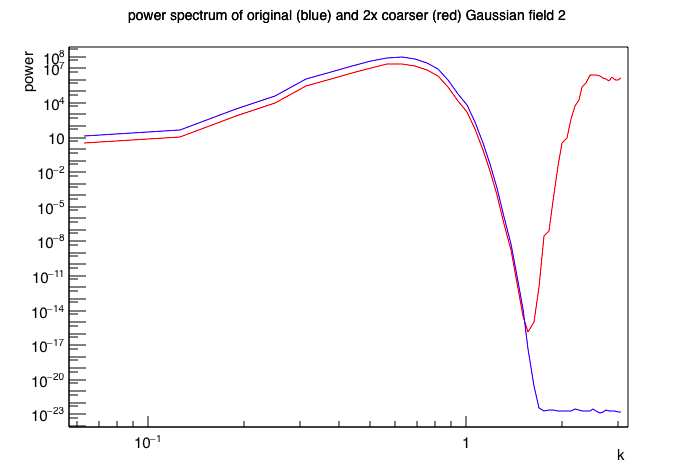
\includegraphics[width=1.1\linewidth]{2BC2}
  \caption{Gaussian2 before and after resampling. Because the original power spectrum is very low beyond new $K^{new}_{Nyquist} =\Pi$/2, aliasing doesn't affect the original  lower spectrum very much. The power spectrum beyond $\Pi$/2, $K^{new}_{Nyquist}$ is no longer meaningful }
  \label{2BC2}
\end{minipage}
\end{figure}



\begin{figure}[!htbp]
\centering
\begin{minipage}{.5\textwidth}
  \centering
  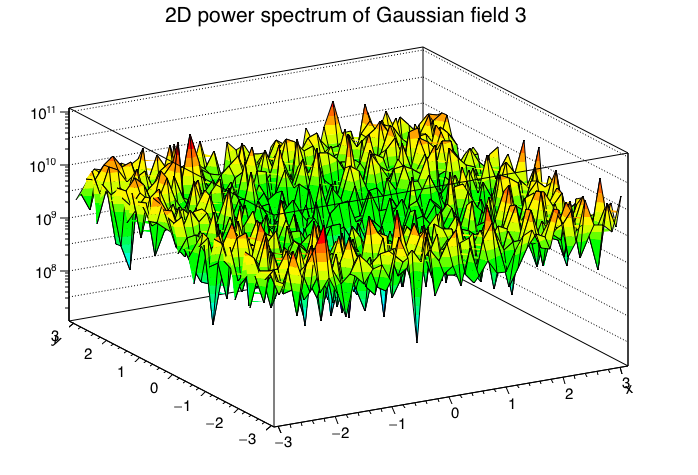
\includegraphics[width=1\linewidth]{gau3color}
  \caption{Gaussian3}
  \label{3col}
\end{minipage}%
\begin{minipage}{.5\textwidth}
  \centering
  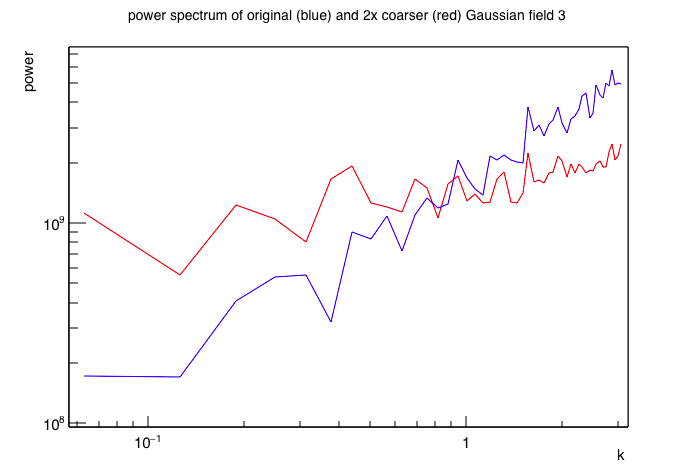
\includegraphics[width=1.1\linewidth]{2BC3}
  \caption{Gaussian3 before and after resampling. Because the original power spectrum is high beyond new $K^{new}_{Nyquist} =\Pi$/2, a lot of power is aliased back into lower frequencies.} 
  \label{2BC3}
\end{minipage}
\end{figure}
\FloatBarrier

 
\subsection{Spectra types}
 \paragraph{}
 Gaussian1 and Gaussian3 field has log-log linear power spectrum in k space with some slope. The power spectrum is a power law of $k^{slope}$.
 \paragraph{}
 Gaussian2 field power spectrum is gaussian.
 

\subsection{Power spectrum of 2 times coarser re-sampled fields}
\paragraph{}
When iterate through the input grid, every other line was skipped. Effectively, the Nyquist frequency is lower by half. Depends on the power spectrum, aliasing affects differently. See more explaination under figures.


\section{Problem 3: Rayleight Levy Random Walk}
\paragraph{}
First, formula for generating random step size r and $\theta$ and 
$\phi$ from uniform random real number [0,1] were derived. 
The accumulative distribution 
\beq
C(r)= \int_{r}^{\infty} P(r)d^3r =  \int_{r_o}^{\infty} P(r)d^3r - \int_{r_o}^{r} P(r)d^3r
\eeq
where $r_0$ is the minimum radial step. The given C(r) and normalization condition gives
\beq
 (\frac{r_o}{r})^\alpha =  1 - \int_{r_o}^{r} P(r)d^3r
\eeq

The last term on the RHS must be a random uniform number between [0,1], say $u_1$. Invert this and use $\alpha$=3/2 one gets:  
\beq r = \frac{r_o}{(1-u_1)^{2/3}} \label{r}  \eeq
The solid angle d$\Omega$ = sin($\theta$)d$\theta$ d$\phi$ distribution must also be uniformly random, requiring dcos($\theta$) and $\theta$ to be uniformly random in [-1,1] and [0,2$\Pi$] respectively. Invert these, one gets: 

\beq \theta = cos^{-1}(2 u_2 -1) \label{theta} \eeq

\beq  \phi = 2 \Pi u_3 \eeq

\paragraph{}
The starting position (x,y,z) is also randomly generated for each run. Increment in x,y,z are then calculated from spherical coordinate transformation. The boundaries are all period (as in a 3-torus).



\subsection{Implementation}
\paragraph{}
See file /comp/hw3/problem3.cc for main code and /root/macros/hw3\_3.cc for plotting
\paragraph{}
See Fig. \ref{walk} for visualization of the random walk

\begin{figure}[!htbp]
  \centering
  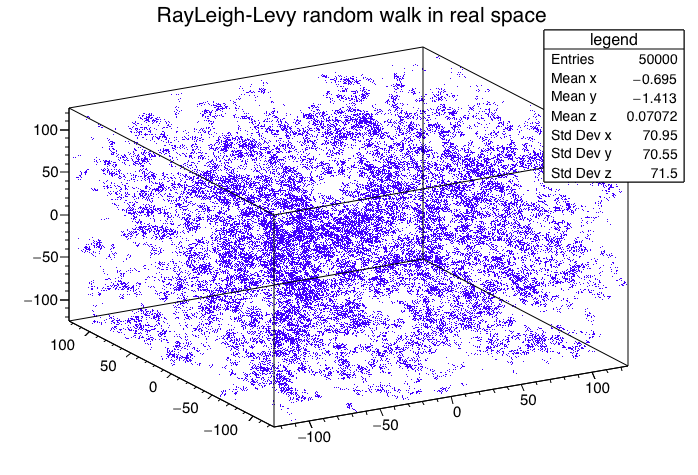
\includegraphics[width=1\linewidth]{walk5000blue}
  \caption{3D plot of the random walk in a periodical cube}
  \label{walk}
\end{figure}
\FloatBarrier


\subsection{CIC algorithm}
\paragraph{}
The code go through all 50000 particles and sort them into cubes of size $s =\frac{250}{400}$. A cube is indexed by the coordinate of the corner closest to the origin $(x_i,y_i,z_i)$, i from 0 to 399. For each particle at (x,y,z), its density value $\delta^3$(x,y,z) is distributed to eight points:
\beq 
(x_i,y_i,z_i),(x_{i+1},y_i,z_i), (i_x,y_{i+1},i_z), (x_{i+1},y_{i+1},z_i)
\eeq
\beq
(x_i,y_i,z_{i+1}),(x_{i+1},y_i,z_{i+1}), (i_x,y_{i+1},z_{i+1}), (x_{i+1},y_{i+1},z_{i+1})
\eeq
where $x_{i+1}-x_{i}$ = s. Since the the boundary is periodic, if i=399, set i+1 $\rightarrow$ 0 instead. The equation for density distributed to point $(x_p, y_p, z_p)$ from 
$\delta^3$(x,y,z)
\beq
f(p)= \frac{s-|x_p-x|}{s} \times \frac{s-|y_p-y|}{s} \times \frac{s-|z_p-z|}{s}
\eeq
each grid point will then receive its density from 8 neighboring random particles.

\subsection{FFT}
\paragraph{}
Use 3D FFTW3 routine. See Fig. \ref{cic} for result.


\subsection{Power Spectrum with and without CIC window correction}
\paragraph{}
Iterate through every one in $400^3$ cubes in k space and obtained its associated k value. 
\paragraph{}
In k space, for every spherical shell of radius k and thickness 2$\Pi$/400, all cubes (aka volume element) belongs to the shell is counted and their Fourier coefficient is distributed to that shell. The total shell contribution/shell volume gives power of k mode.
\paragraph{}
The FFT of the Window function is
\begin{equation}
\hat{W} = \hat{W_x} \hat{W_y} \hat{W_z}
\end{equation}
where for $k_{x_i}}$ non zero
\beq
\hat{W_{x_i}}= \frac{sin^2(k_{x_i}s/2)}{(k_{x_i}s/2)^2} ; x_i = x, y, z
\eeq
and for $k_{x_i}$ =0, $\hat{W_{x_i}}=1$

\begin{figure}[!htbp]
  \centering

  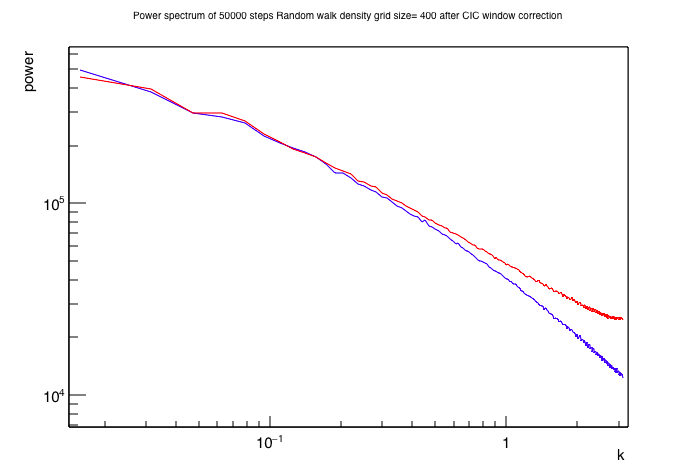
\includegraphics[width=1\linewidth]{finalofall}
  \caption{Power spectrum of the random walk before (blue) and after (red) applying CIC window correction. K space 400x400x400}
  \label{cic}
\end{figure}
  
\begin{figure}[!htbp]

    \centering
  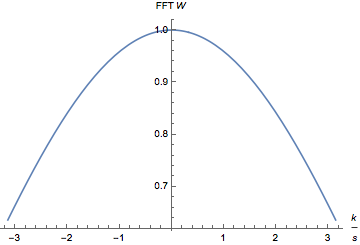
\includegraphics[width=0.4\linewidth]{Window}
  \caption{The 1D $\hat{W}$ Function approach 1 as k approach 0 but become small as k approach Nyquist value}
  \label{win}

\end{figure}
\FloatBarrier



\begin{figure}[!htbp]
  \centering
  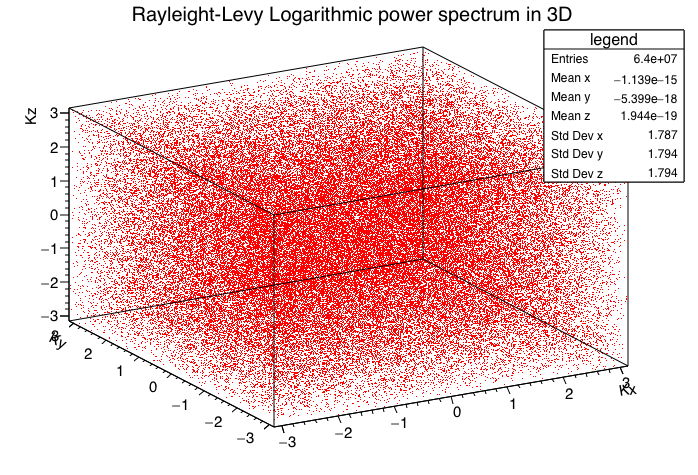
\includegraphics[width=1\linewidth]{3D_555_log}
  \caption{Log of power spectrum of in K space after window correction}
  \label{fig:test2}
\end{figure}
\FloatBarrier

\subsection{Explanation}
\paragraph{}
Power spectrum of higher frequencies near Nyquist value ($\Pi$) are amplified more after convoluting with the window function. Mathematically the correction  $\frac{1}{\hat{W}}$ increases as k approach Nyquist value so the correction for  $|\hat{f}|$ is stronger in this regime. As k approaches 0, the correction $\frac{1}{\hat{W}}$ approaches 1 when the original spectrum is unaffected. See Fig. (\ref{win})

\paragraph{}
(More figures below)


\begin{thebibliography}{9}


\bibitem{Beck}
  Roman Scoccimarro,
  \emph{Lecture notes}. 2015
  \label{roman}
\end{thebibliography}
\end{document}


